\documentclass[10pt,a4paper,UTF8]{ctexart}
\usepackage{geometry}%用于设置上下左右页边距
	\geometry{left=2.5cm,right=2.5cm,top=3.2cm,bottom=2.8cm}
\usepackage{xeCJK,amsmath,paralist,enumerate,booktabs,multirow,graphicx,subfig,setspace,listings,lastpage,hyperref}
\usepackage{amsthm, amssymb, bm, color, framed, graphicx, hyperref, mathrsfs}
\usepackage{mathrsfs}  
	\setlength{\parindent}{2em}
	\lstset{language=Matlab}%
\usepackage{fancyhdr}
\usepackage{graphicx}
\usepackage{listings}
\usepackage{xcolor}
\usepackage{float}

\definecolor{mKeyword}{RGB}{0,0,255}          % bule
\definecolor{mString}{RGB}{160,32,240}        % purple
\definecolor{mComment}{RGB}{34,139,34}        % green
\definecolor{mNumber}{RGB}{128,128,128} 

\lstdefinestyle {njulisting} {
	basewidth = 0.5 em,
	lineskip = 3 pt,
	basicstyle = \small\ttfamily,
	% keywordstyle = \bfseries,
	commentstyle = \itshape\color{gray}, 
	basicstyle=\small\ttfamily,
	keywordstyle={\color{mKeyword}},     % sets color for keywords
	stringstyle={\color{mString}},       % sets color for strings
	commentstyle={\color{mComment}},     % sets color for comments
	numberstyle=\tiny\color{mNumber},
	numbers = left,
	captionpos = t,
	breaklines = true,
	xleftmargin = 2 em,
	xrightmargin = 2 em,
	frame=tlrb,
	tabsize=4
}

\lstset{
style = njulisting, % 调用上述样式 
flexiblecolumns % 允许调整字符宽度
}

\pagestyle{fancy}
\lhead{\textsc{Foundation of Computing System}}
\rhead{\textsc{Nanjing University}}
\cfoot{\thepage}
\renewcommand{\headrulewidth}{0.4pt}
\renewcommand{\theenumi}{(\arabic{enumi})}


\definecolor{shadecolor}{RGB}{241, 241, 255}

\newcommand{\problemname}{待定义}
\newenvironment{problem}{\begin{shaded}\par\noindent\textbf{题目\  \problemname}}{\end{shaded}\par}
\newenvironment{solution}{\par\noindent\textbf{解答}\ }{\par}
\newenvironment{note}{\par\noindent\textbf{题目 \problemname 的注记}}{\par}

\begin{document}

\begin{center}
\LARGE\textbf{第十六章习题参考答案}
\end{center}

{\kaishu 包含题目:习题$16.1$、$16.2$、$16.9$、$16.10$和$16.14$}

\renewcommand{\problemname}{16.1}
\begin{problem}
	对于如下程序:
	\begin{lstlisting}[language=C]
#include <stdio.h> 
int main() { 
	int x = 1;	
	int *ptr1; 
	int **ptr2;

  	ptr2 = &ptr1; 
	*ptr2 = &x; 
	**ptr2 = 2; 

	x++; 
	(*ptr1)++; 
	(**ptr2)++; 

  	printf ("%d\n", x); 
} 
	\end{lstlisting}
	\begin{enumerate}[(1)]
		\item 程序的输出是什么?提示:\verb|ptr2| 是一个指向指针的指针。
		\item 请描述语句 \verb|(**ptr2)++;| 执行之后的运行时栈中的内容。	
	\end{enumerate}
\end{problem}

\begin{solution}
	\begin{enumerate}[(1)]
		\item 5[空格][换行]
		\item 如图所示
		\begin{figure}[H]
				\centering
				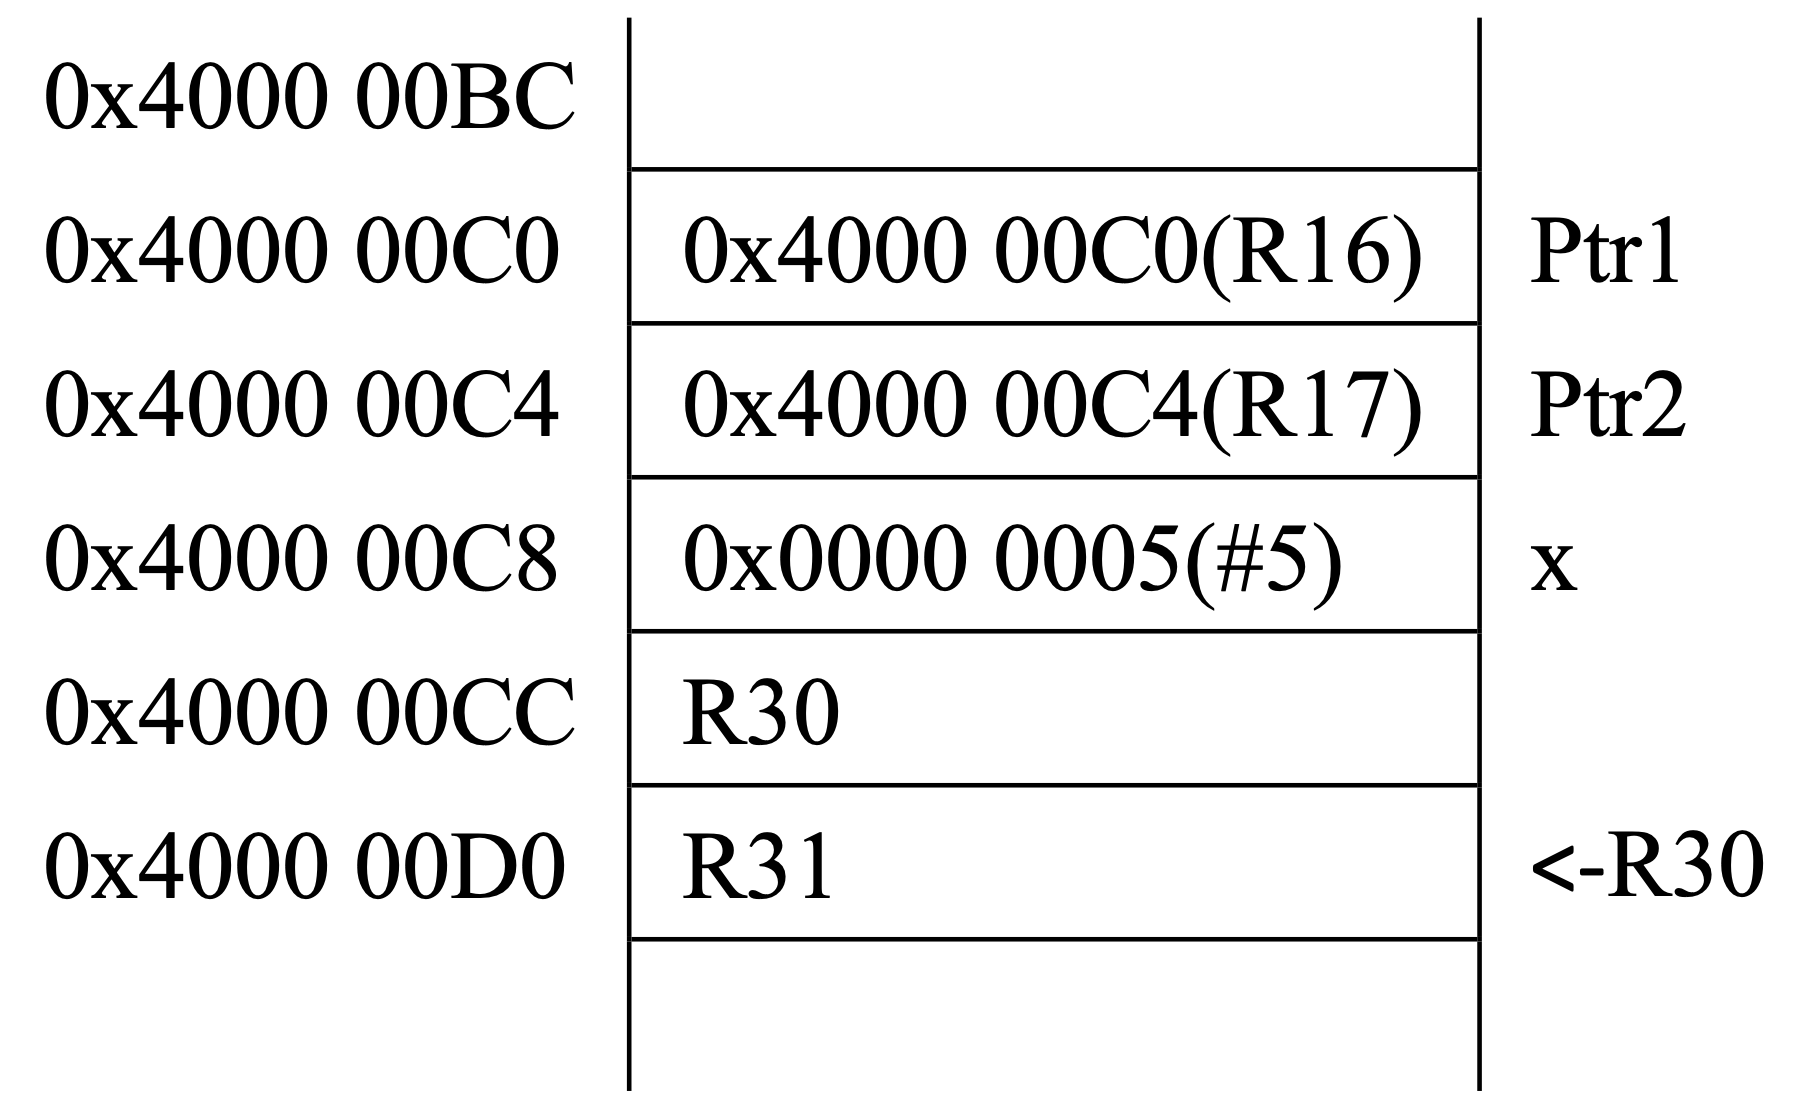
\includegraphics[scale=0.2]{img/16.1}
		\end{figure}
	\end{enumerate}
\end{solution}


\renewcommand{\problemname}{16.2}
\begin{problem}
	下列代码片段的输出是什么?
	\begin{enumerate}[(1)]
		\item \ \begin{lstlisting}[language=C]
char ch[7] = "1a2b3c"; 
int i, s = 0; 
for (i = 0; i < 6; i++) { 
	if (ch[i] >= '0' && ch[i] <= '9') 
		s = s + ch[i] - '0'; 
	else 
		s = s + ch[i] - 'a'; 
} 
printf ("%d\n", s); 
		\end{lstlisting}
		\item \ \begin{lstlisting}[language=C]
char str[13] = "hello world!"; 
char *p; 
p = str; 
while (*p != ' ') { 
	printf ("%c", *p - 'a' + 'A'); 
	p++; 
}
		\end{lstlisting}
	\end{enumerate}
\end{problem}

\begin{solution}
	\begin{enumerate}[(1)]
		\item 9[换行]
		\item HELLO
	\end{enumerate}
\end{solution}


\renewcommand{\problemname}{16.9}
\begin{problem}
	将函数 \verb|StringLength| 翻译为DLX汇编语言。
	\begin{lstlisting}[language=C]
int StringLength (char string[]) { 
int index = 0; 
while (string[index] != '\0') 
	index = index + 1; 
return index; 
} 
	\end{lstlisting}
\end{problem}

\begin{solution}
	\begin{lstlisting}[language=C]
StringLength:	subi	r29, r29, #4 
				sw		0(r29), r16	; 	压入r16(寄存器的保存) 
				addi	r16, r0, #0	; 	r16 <- index
LOOP:			addi 	r9, r4, r16	; 	计算string[index]的地址值 
				lb		r10, 0(r9) 	; 	r10 <- string[index]
				beqz 	r10, EXIT
				addi	r16, r16, #1; 	index = index + 1
				J 		LOOP
EXIT:			addi 	r2, r16, #0	; 	return index
				lw		r16, 0(r29)	; 	r16出栈
				addi	r29, r29, #4 
				ret 

	\end{lstlisting}
	R8$\sim$R15和R24、R25用于存放临时产生的值,R16$\sim$R23用于存放局部变量。
\end{solution}


\renewcommand{\problemname}{16.10}
\begin{problem}
	如下代码从键盘读入一个字符串,将其中的小写字母转换为大写字母后输出。
	代码中存在bug,请找出并修复。
	\begin{lstlisting}[language=C]
#include <stdio.h> 

char *ToUpper (char *inchar); 
		
int main () { 
	char str[10]; 
	printf ("Enter a string : "); 
	scanf ("%s", str); 
	printf ("%s \n", ToUpper (str) ); 
} 

char *ToUpper (char *inchar) { 
	char str[10]; 
	int i = 0; 
	while (*(inchar + i) != '\0') { 
		if ('a' <= *(inchar + i) && *(inchar + i) <= 'z') 
			*(str + i) = *(inchar + i) - ('a' - 'A'); 
		else 
			*(str + i) = *(inchar + i); 
		i++; 
	} 
	return str; 
} 	
	\end{lstlisting}
\end{problem}

\begin{solution}
	该程序的bug为:\verb|ToUpper| 函数中返回值是一个局部变量的指针,离开该函数后指针所指的内容即为非法;
	根据题意可知,返回值应该仍然是输入参数。

	解决方案:将 \verb|char str[10];| 改为 \verb|char *str = inchar;| 即可。
\end{solution}


\renewcommand{\problemname}{16.14}
\begin{problem}
	如果输入流为 \verb|abc123 def|

	对于如下函数调用,字符数组x的值将是什么?
	\begin{lstlisting}[language=C]
scanf("%s", x)
	\end{lstlisting}
\end{problem}

\begin{solution}
	字符数组x中的值未发生改变,如果x声明时为初始化,将会是垃圾数据。
\end{solution}

\end{document}
